%!TEX root = Vorlage_Buch.tex
\chapter{Leckeres aus dem Holzbackofen}\label{Chapter4}
\lettrine[lines=3]{D}{er Holzbackofen} ist eine echte Bereicherung für das 
Outdoor-Kochvergnügen.
Die Einsatzmöglichkeiten sind schier unerschöpflich. Fast alles das auf
dem Herd oder dem Grill gemacht wird, ist auch im Backofen möglich. Ob
Fleisch, Fisch, Gemüse, Pizzen, Brote oder Desserts das alles gelingt im 
Holzbackofen. Der Kreativität wird keine Grenzen gesetzt. Das Charmante an
dieser Zubereitungsmethode ist die lange Haltezeit der Temperatur. Pizzen
werden jenseits der 300 ℃ gebacken, danach kann locker noch ein 
Holzofenbrot gebacken werden. So kann die Restwärme noch sinnvoll genutzt
werden.

\begin{figure}[htbp]
	\centering
	\begin{minipage}{1\textwidth}
		\centering
		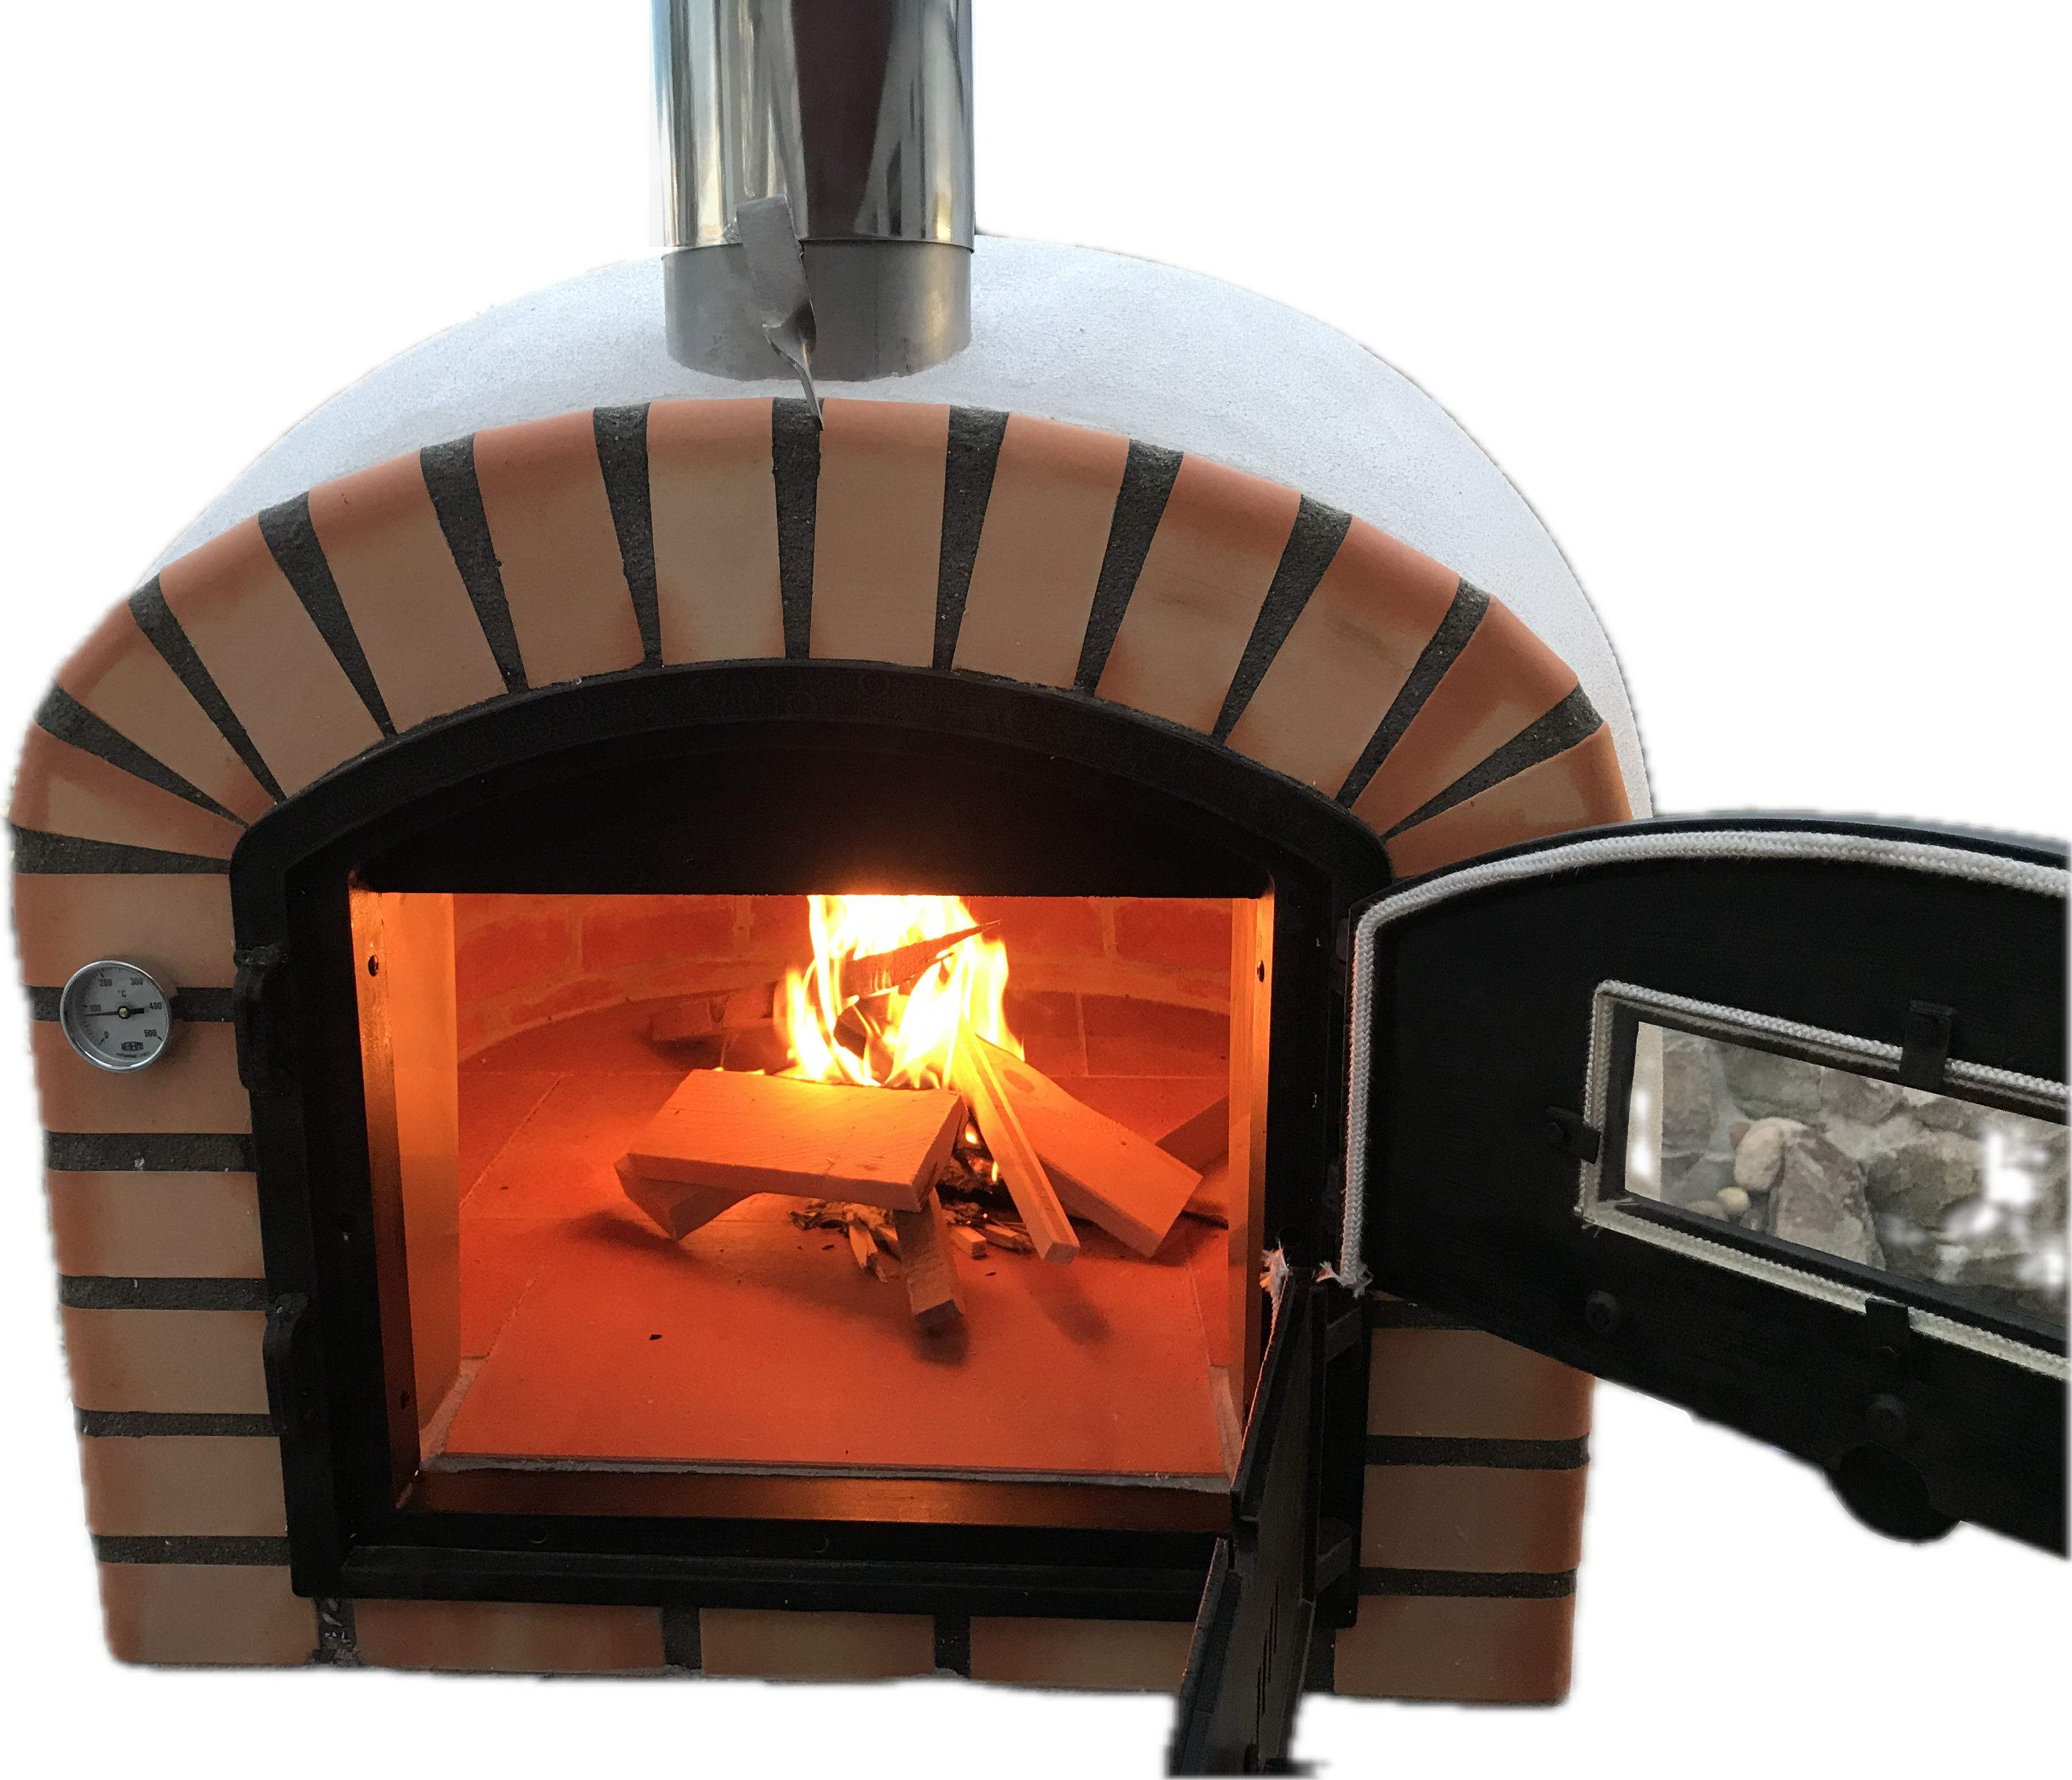
\includegraphics[width=.9\linewidth]{pics/Backofen}
		\captionof{figure}{HolzBackofen}
		\label{fig:Backofen}
	\end{minipage}
\end{figure}
\newpage

\section{Teige und was sich daraus machen lässt}

\subsection{Eine echt leckere Pizza}

\paragraph{Zutaten Teig}

\begin{itemize}[noitemsep]
	\item 1 kg Mehl (Type 00 mit mindestens 12\% Eiweiß)
	\item 650 g kaltes Leitungswasser (Anfänger 600 g, weil leichter zu 
	verarbeiten)
	\item 25 g feines Salz
	\item 15 g Olivenöl
	\item 2 g frische Hefe
\end{itemize} 

\paragraph{Zutaten Pizzasoße}
 
\begin{itemize}[noitemsep]
	\item 500 g frische Tomaten
	\item 500 g passierte Tomaten aus der Flasche (hier von Mutti)
	\item 2 große Zwiebeln
	\item 2 Stück chinesischer Knoblauch
	\item 50 ml Olivenöl
	\item Salz
	\item je nach Geschmack Kräuter
\end{itemize}

\paragraph{Zubereitung }
Das Mehl in einer Rührschüssel vorlegen. Von dem Wasser ca. 100 ml 
abnehmen um die Hefe aufzulösen. Den Rest des Wassers zu dem Mehl 
geben 
und das Ganze mit einem Kochlöffel verrühren bis das gesamte Wasser 
aufgenommen wurde. Den Teig  abdecken und 30 Minuten ruhen lassen. Nach 
dem Ruhen das Olivenöl und das Wasser mit der aufgelösten Hefe zugeben und 
alles kneten, bis das Wasser und das Öl aufgenommen wurde, nun das Salz 
zugeben und den Teig fertig kneten ca. 15 Minuten. Da kann natürlich auch in 
einer Küchenmaschine erledigt werden. Knetzeit ca. 6 Minuten bei mittlerer 
Geschwindigkeit.
Den Teig in der Rührschüssel belassen und diese mit Frischhaltefolie 
verschließen. Den Teig 24 Stunden im Kühlschrank gehen lassen. Den Teig 
nach 24 Stunden aus der Schüssel nehmen, kurz durchkneten und in 6 
gleichmäßige Teiglinge teilen. Die Teiglinge zu Kugeln formen, in eine 
Auflaufform legen, diese mit Frischhaltefolie verschließen und nochmals 24 
Stunden im Kühlschrank gehen lassen. 

\paragraph{Zubereitung Tomatensoße}
Die Zwiebeln klein schneiden und im Olivenöl andünsten, nach einiger Zeit den 
gehackten Knoblauch zugeben. In der Zwischenzeit die frischen Tomaten in 
Stücke schneiden und zusammen mit den passierten Tomaten zu den 
angedünsteten Zwiebeln geben und köcheln lassen bis die Tomaten verkocht 
sind. Je nach Geschmack die Soße stückig lassen oder durch ein Sieb streichen.
Falls gewünscht Kräuter zugeben und mit Salz abschmecken.

\paragraph{Zubereitung Pizza}
Die Teiglinge aus der Form nehmen und von der Mitte heraus flach drücken, 
darauf achten, dass die Luft nicht aus den Rand gedrückt wird. Wenn der Boden 
die richtige Größe hat mit Tomatensoße bestreichen, nach Belieben belegen 
und bei mindestens 300°C im Holzbackofen backen.
\newpage

\begin{figure}[htbp]
	\centering
	\begin{minipage}{1\textwidth}
		\centering
		\includegraphics[width=1\linewidth]{pics/Pizza}
		\captionof{figure}{Pizza aus dem Holzbackofen}
		\label{fig:Pizza}
	\end{minipage}
\end{figure}
\newpage
